\documentclass[a4paper,12pt]{article}

\usepackage[utf8]{inputenc}
\usepackage[T1]{fontenc}
\usepackage[polish]{babel}
\usepackage{amsmath, amssymb}
\usepackage{graphicx}
\usepackage{float}
\usepackage{hyperref}
\usepackage{geometry}
\usepackage{csvsimple} 

\geometry{margin=2.5cm}

\title{Sprawozdanie 1 z Statystyki i Modeli Liniowych}
\author{Wiktor Zoga}
\date{\today}

\begin{document}

\maketitle
\newpage

\section{Zadanie 1 - Porównywanie estymatorów}

\subsection{Opis eksperymentu}
W tym zadaniu do próby wielkości $n-1=49$ z rozkładu $N(0, 1)$ dodano kolejne wartości $k=10, 20, ..., 100$

Na tej podstawie wyliczone dwa estymatory:

\begin{itemize}
    \item $\hat{\theta}_1$ -- średnia arytmetyczna
    \item $\hat{\theta}_2$ -- mediana
\end{itemize}

Doświadczenie powtórzono $10{,}000$ razy dla każdego zestawu z $k$. 
Błąd średniokwadratowy, obciążenie i wariancja zostały przedstawione na wykresie w zależności od parametru k.

\section{Wyniki}

\begin{figure}[H]
    \centering
    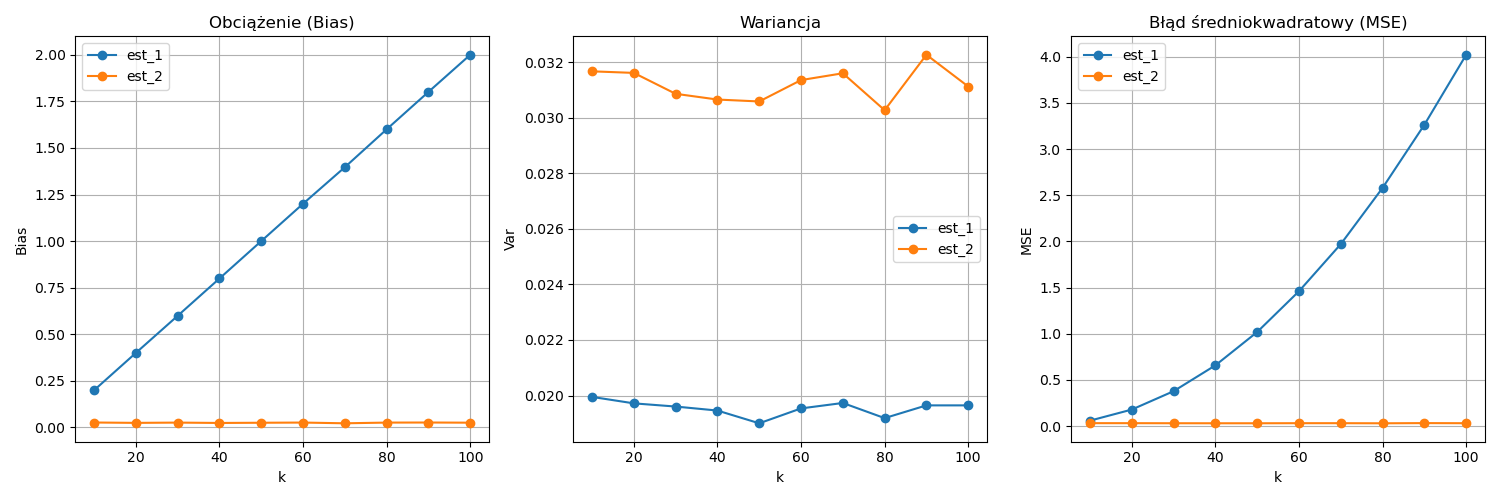
\includegraphics[width=1.1\textwidth]{../plots/plot.png}
    \caption{Wykres kolejnych statystyk w zależności od parametru k.}
\end{figure}

\section{Dyskusja Wyników}

Eksperyment ten, polegający na wprowadzeniu pojedynczej obserwacji odstającej $k$ do próby z rozkładu $\mathcal{N}(0,1)$, w sposób jednoznaczny ilustruje pojęcie \textbf{odporności} estymatorów na obserwacje odstające.

\subsection*{Analiza Estymatora $\hat{\theta}_1$ (Średnia Arytmetyczna)}

Średnia arytmetyczna jest estymatorem znanym ze swojej wrażliwości na wartości ekstremalne. Przy stosunkowo niewielkiej próbie ($n=50$), wpływ pojedynczego punktu $k$ jest znaczący.

\begin{itemize}
    \item \textbf{Obciążenie:} Teoretyczne obciążenie średniej w tym eksperymencie wynosi:
    \[ \text{Bias}(\hat{\theta}_1) = E[\hat{\theta}_1] - \theta = E\left[ \frac{1}{n} \left(\sum_{i=1}^{n-1} X_i + k\right) \right]\]
    \[ \text{Bias}(\hat{\theta}_1) = \frac{1}{n} \left( \sum_{i=1}^{n-1} E[X_i] + k \right) = \frac{k}{n} \]
    Dla $n=50$, obciążenie wynosi $k/50$. Jest to funkcja \textbf{idealnie liniowo rosnąca} wraz ze wzrostem $k$, co powinno być widoczne na wykresach z symulacji.

    \item \textbf{Wariancja:} Co ciekawe, wariancja estymatora $\hat{\theta}_1$ nie jest zaburzona przez anomalię, ponieważ wariancja jest niezmiennicza względem przesunięcia:
    \[ \text{Var}(\hat{\theta}_1) = \text{Var}\left( \frac{1}{n} \left(\sum_{i=1}^{n-1} X_i + k\right) \right) = \frac{1}{n^2} \left( \sum_{i=1}^{n-1} \text{Var}(X_i) \right) \]
    \[ \text{Var}(\hat{\theta}_1) = \frac{1}{n^2} ( (n-1) \cdot 1 + 0 ) = \frac{n-1}{n^2} \]
    Dla $n=50$, wariancja jest stała i wynosi $49/2500 \approx 0.0196$, niezależnie od wartości $k$.

    \item \textbf{MSE:} Ponieważ $\text{MSE} = \text{Var} + \text{Bias}^2$:
    \[ \text{MSE}(\hat{\theta}_1) = \frac{n-1}{n^2} + \left(\frac{k}{n}\right)^2 = \frac{n-1 + k^2}{n^2} \]
    Wartość MSE jest zdominowana przez obciążenie i rośnie \textbf{kwadratowo} wraz ze wzrostem $k$.
\end{itemize}

\subsection*{Analiza Estymatora $\hat{\theta}_2$ (Mediana)}

Mediana jest klasycznym przykładem estymatora odpornego na obserwacje odstające.
\begin{itemize}
    \item Dopóki obserwacja odstająca $k$ jest wartością ekstremalną (co ma miejsce dla $k \ge 10$), będzie ona po prostu zajmować ostatnią pozycję $X_{(50)}$ i \textbf{nie będzie miała żadnego wpływu} na wyznaczenie wartości centralnych.
    \item W rezultacie, zarówno \textbf{obciążenie}, \textbf{wariancja}, jak i \textbf{MSE} estymatora $\hat{\theta}_2$ pozostają praktycznie \textbf{stałe} i niewrażliwe na wzrost $k$.
\end{itemize}

\subsection*{Wnioski}
Symulacje jednoznacznie potwierdzają teoretyczne przesłanki, że mediana jest estymatorem znacznie bardziej odpornym na ekstremalne obserwacje odstające niż średnia arytmetyczna.

\end{document}
